%% ----------------------------------------------------------------
%% SETTINGS
%% ----------------------------------------------------------------
\documentclass[../et.tex]{subfiles}

%% ----------------------------------------------------------------
%% BEGIN
%% ----------------------------------------------------------------
\begin{document}

%% ----------------------------------------------------------------
%% DOCUMENT
%% ----------------------------------------------------------------
La etapa de generación de corriente se implementará utilizando una configuración puente H, utilizando MOSFETs controlados por sus respectivos drivers. En las Figuras \ref{fig:mosfet} y \ref{fig:mosfet-driver} se pueden observar los dispositivos y sus respectivos esquemáticos que se utilizarán. Se deberá incluír un circuito de alimentación, mostrado en la \autoref{fig:mosfet-alimentacion}, un circuito de protección, mostrado en la \autoref{fig:mosfet-proteccion} y una resistencia de medición tipo shunt, junto con un conector para la salida al multiplicador, mostrados en la \autoref{fig:mosfet-shunt}.

Se utilizarán cuatro MOSFETs junto con dos drivers, con la misma configuración mostrada.

\begin{figure}[!htbp]
  \centering
  \begin{subfigure}[b]{0.4\textwidth}
    \centering
    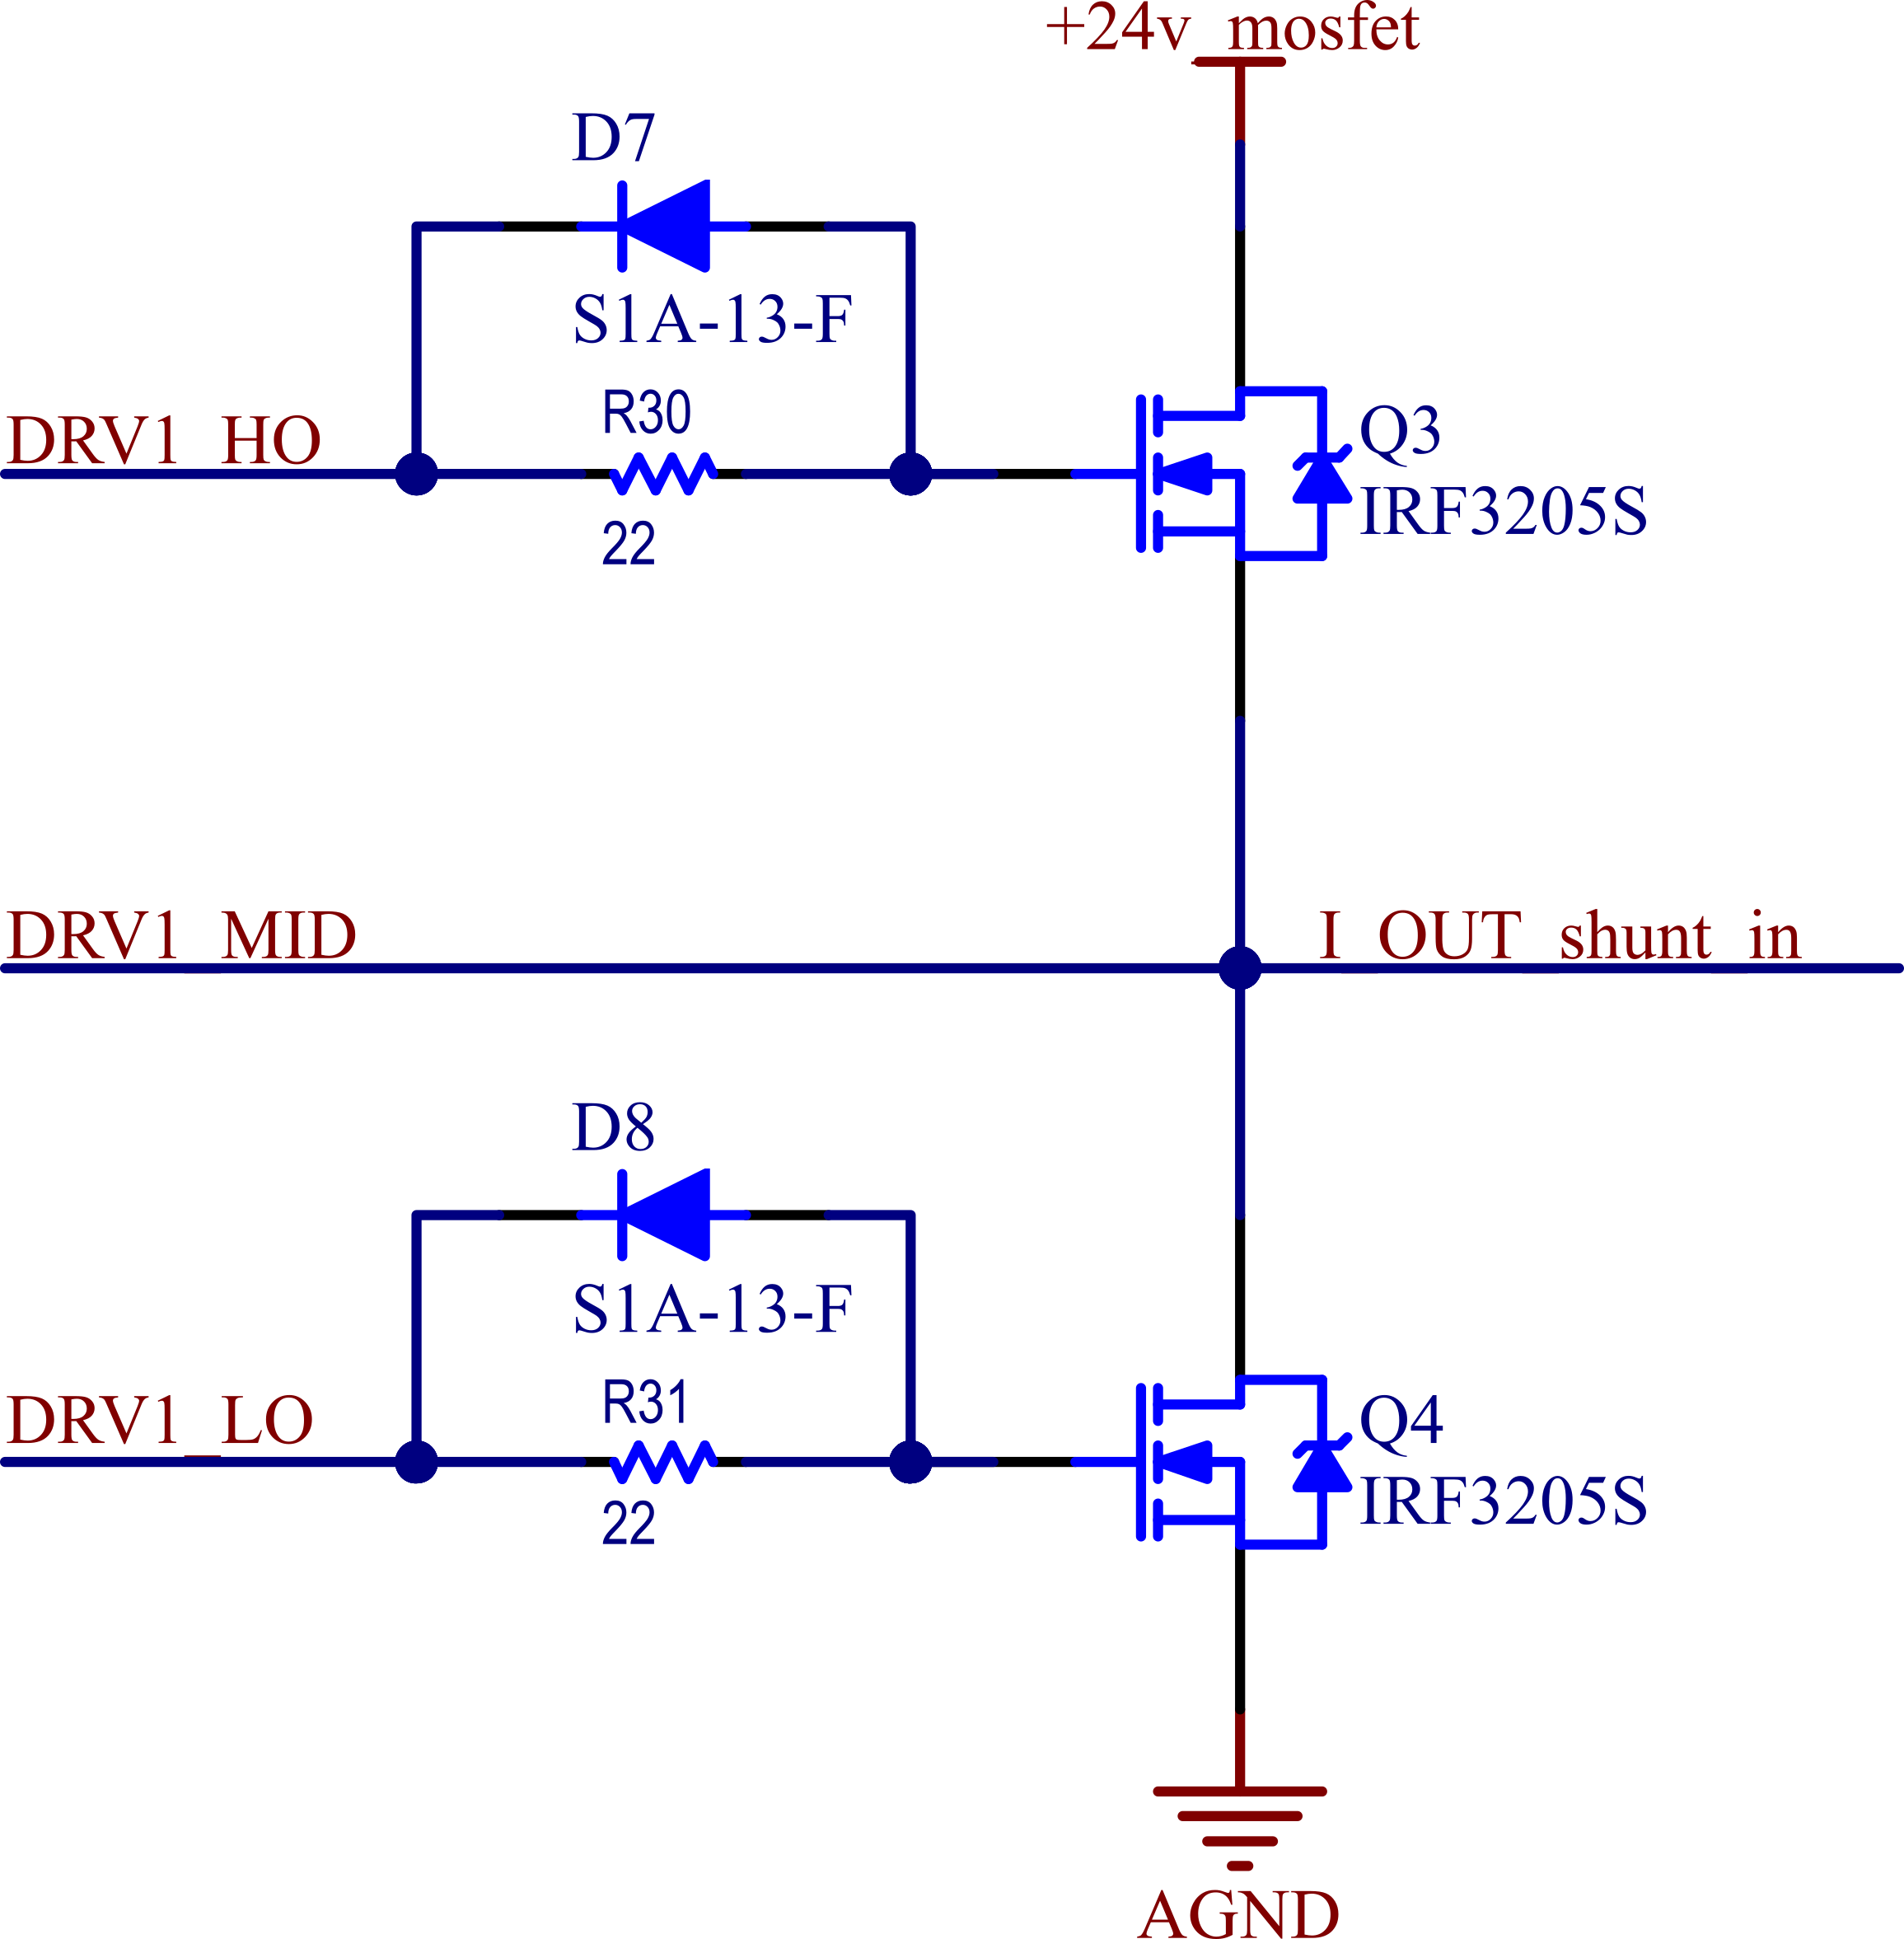
\includegraphics[width=\textwidth]{../images/mosfet.png}
    \caption{Esquemático MOSFETs}
    \label{fig:mosfet}
    \vspace*{10mm}
  \end{subfigure}
  \hfill
  \begin{subfigure}[b]{0.55\textwidth}
    \centering
    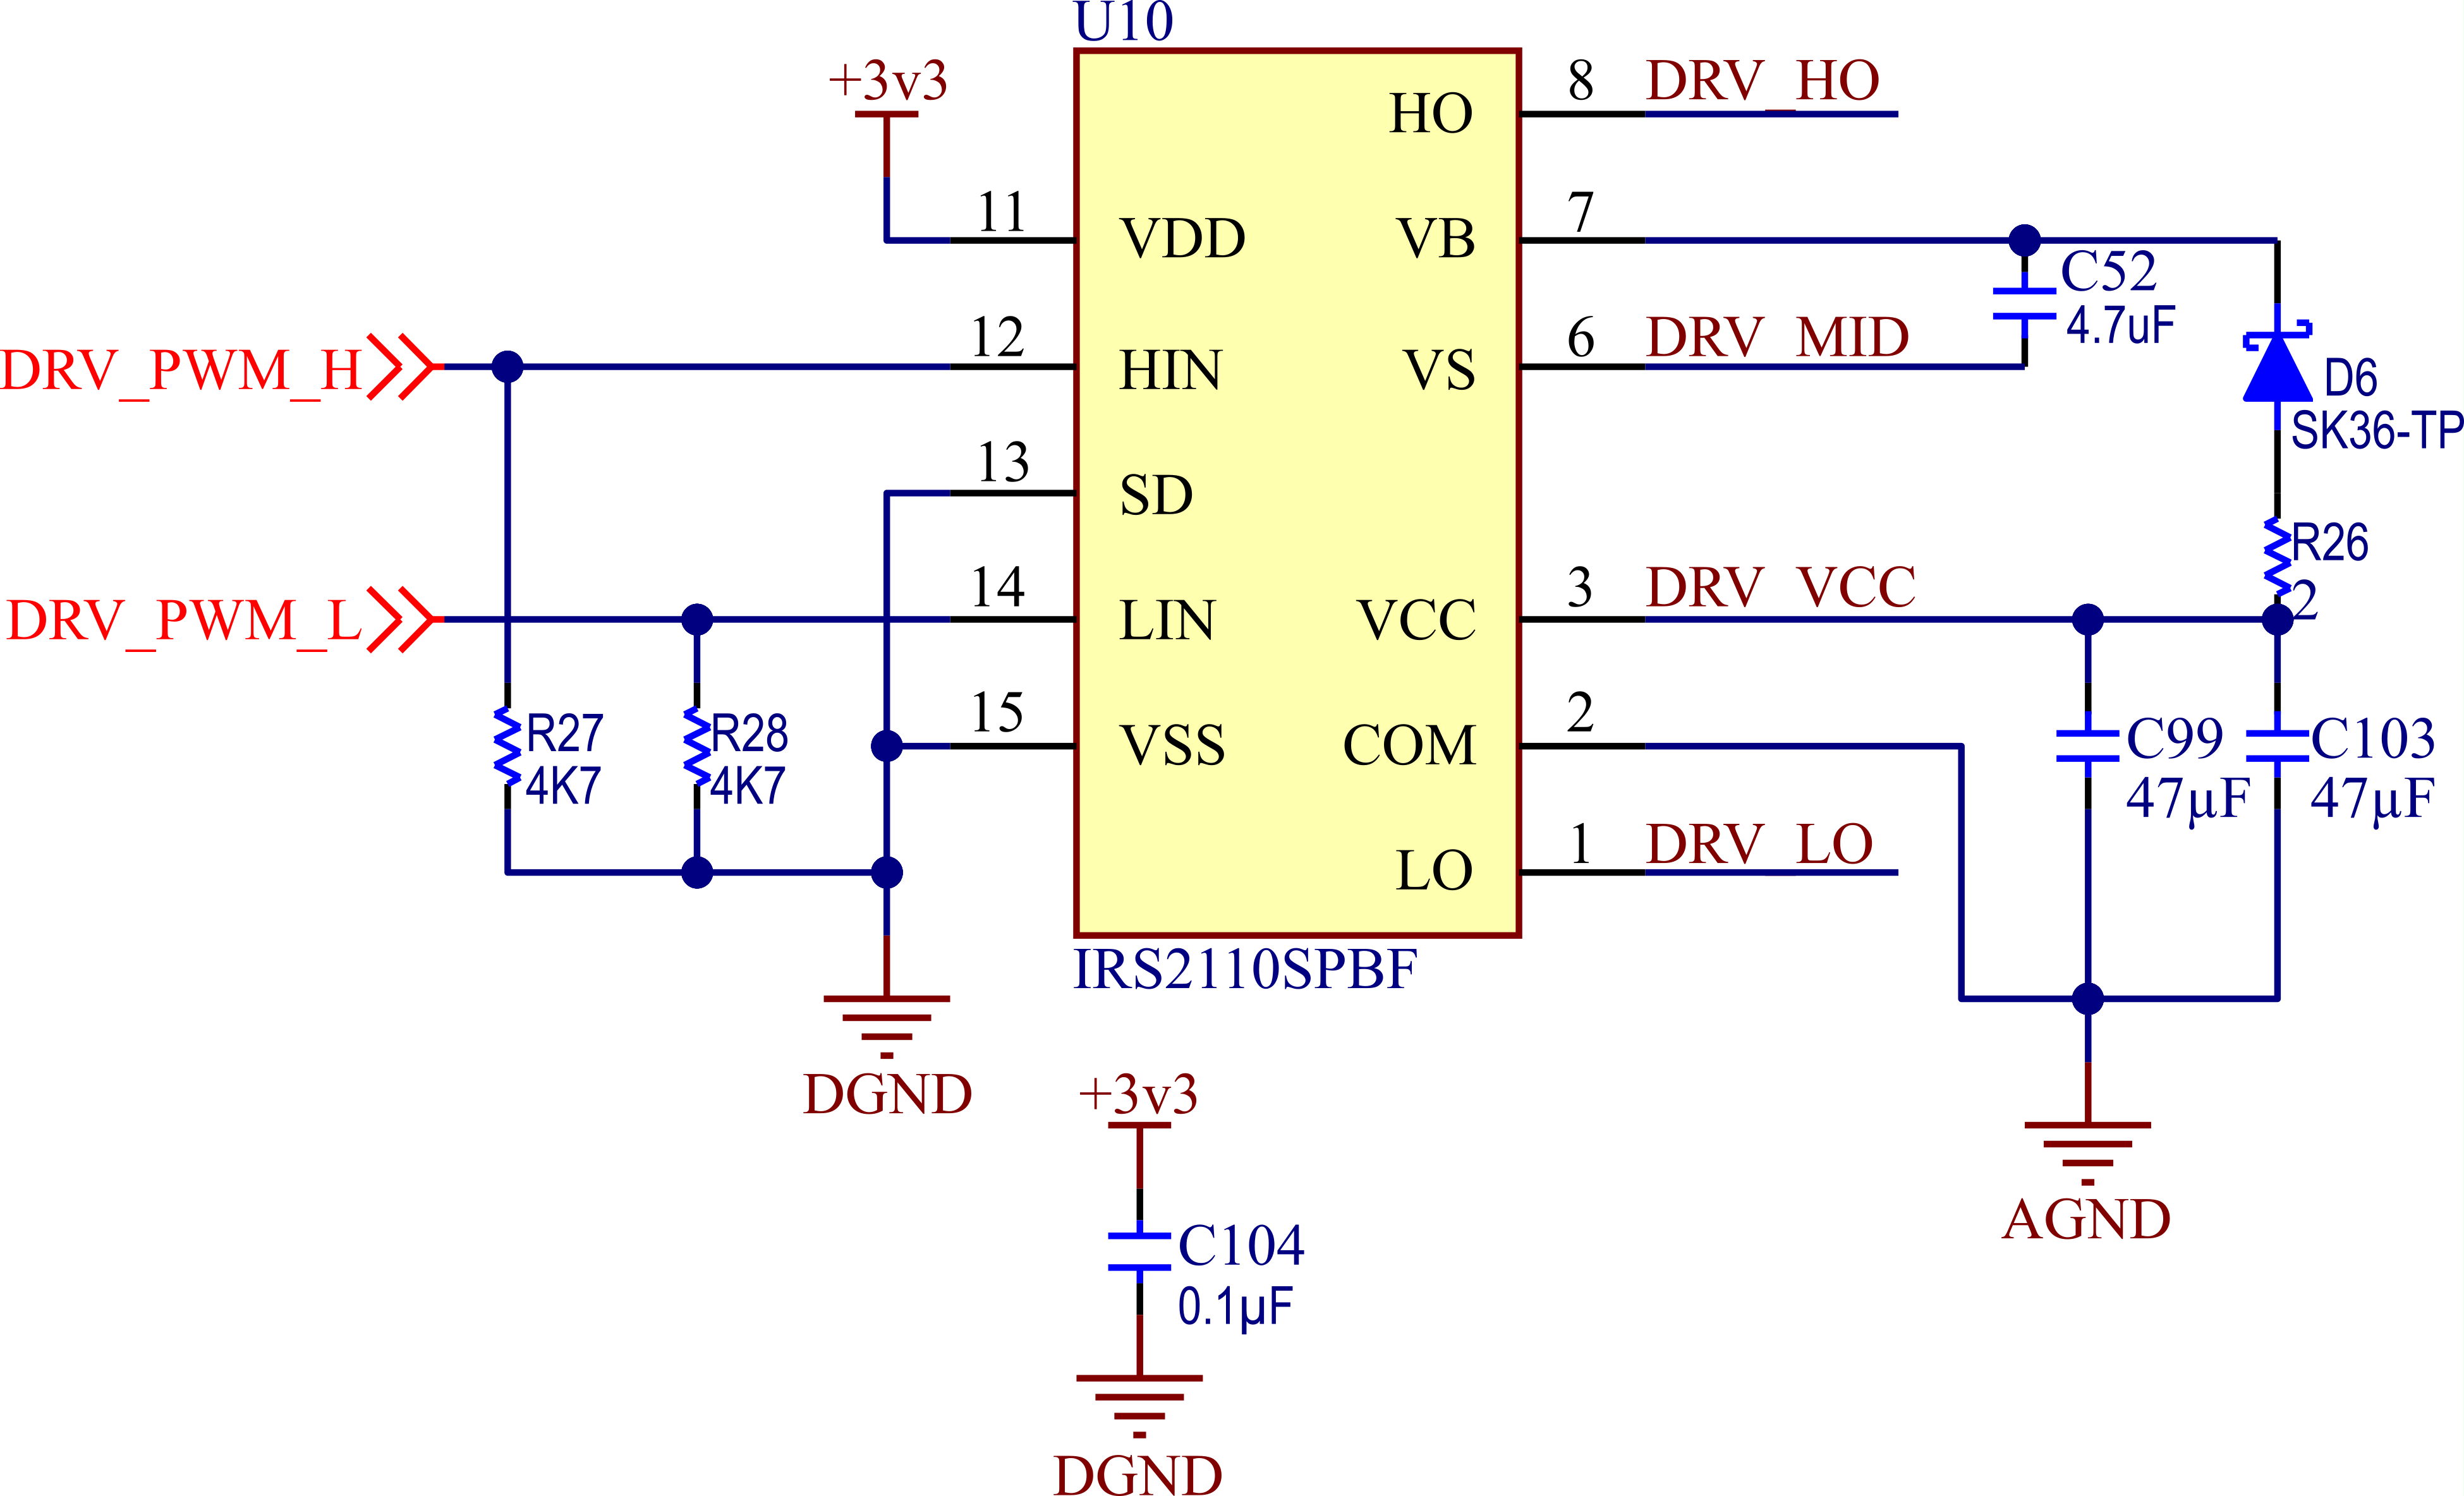
\includegraphics[width=\textwidth]{../images/mosfet-driver.png}
    \caption{Esquemático MOSFET Driver}
    \label{fig:mosfet-driver}
    \vspace*{10mm}
  \end{subfigure}

  \begin{subfigure}[b]{0.4\textwidth}
    \centering
    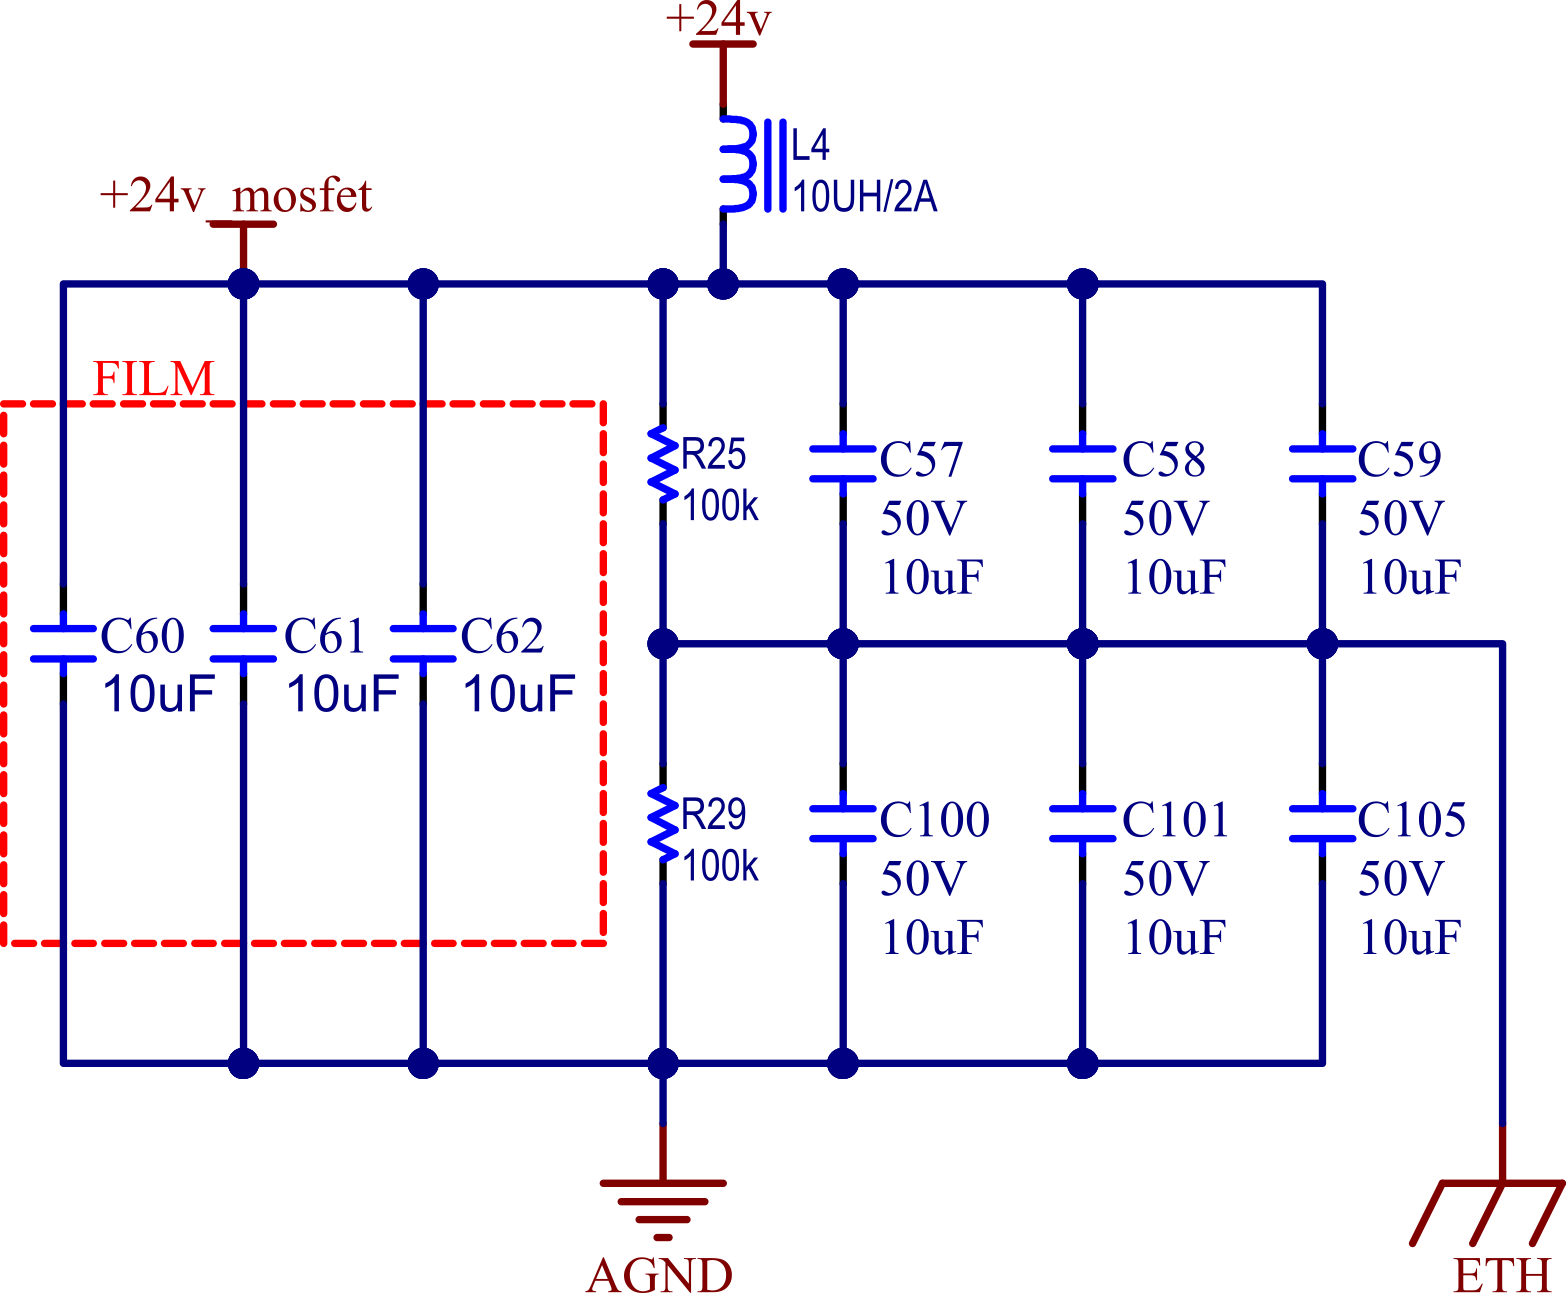
\includegraphics[width=\textwidth]{../images/mosfet-alimentacion.png}
    \caption{Esquemático alimentacion MOSFETs}
    \label{fig:mosfet-alimentacion}
    \vspace*{10mm}
  \end{subfigure}
  \hfill
  \begin{subfigure}[b]{0.5\textwidth}
    \centering
    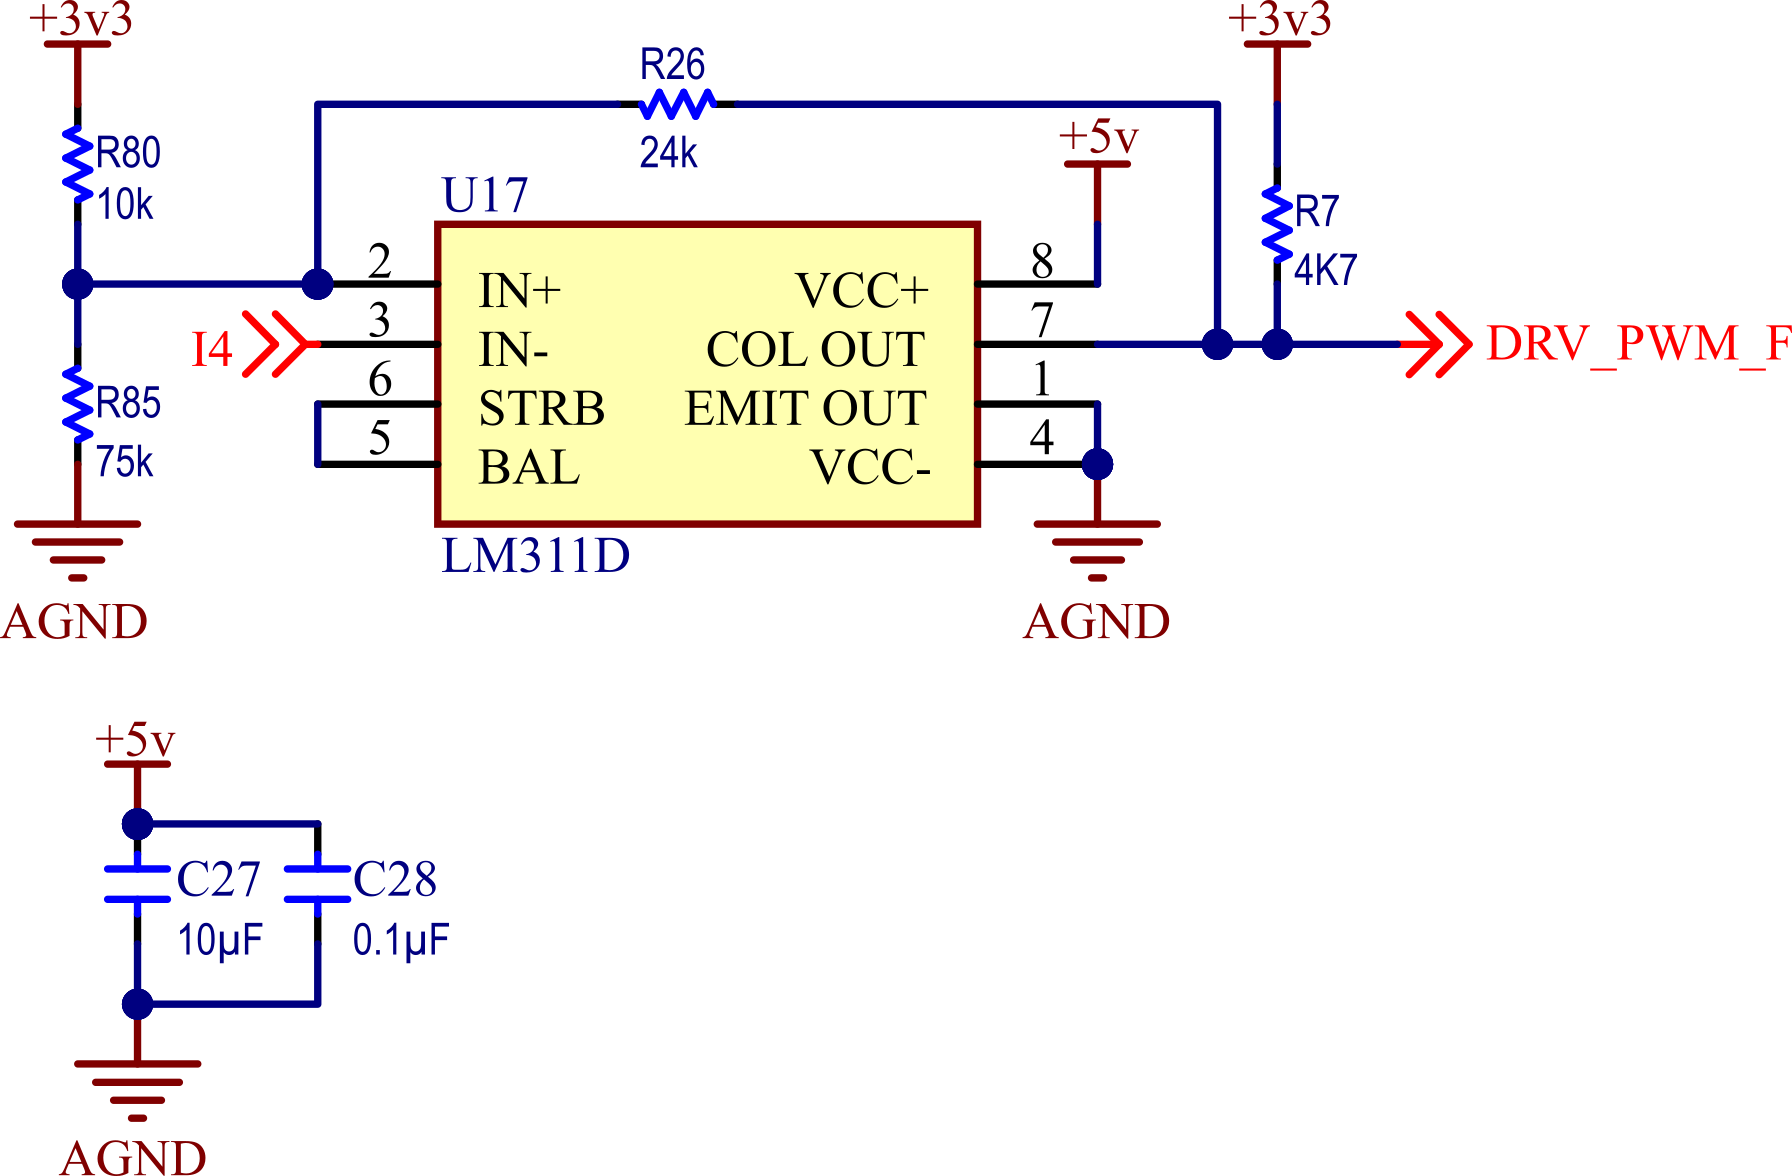
\includegraphics[width=\textwidth]{../images/mosfet-proteccion.png}
    \caption{Esquemático protección MOSFETs}
    \label{fig:mosfet-proteccion}
    \vspace*{10mm}
  \end{subfigure}

  \begin{subfigure}[b]{0.4\textwidth}
    \centering
    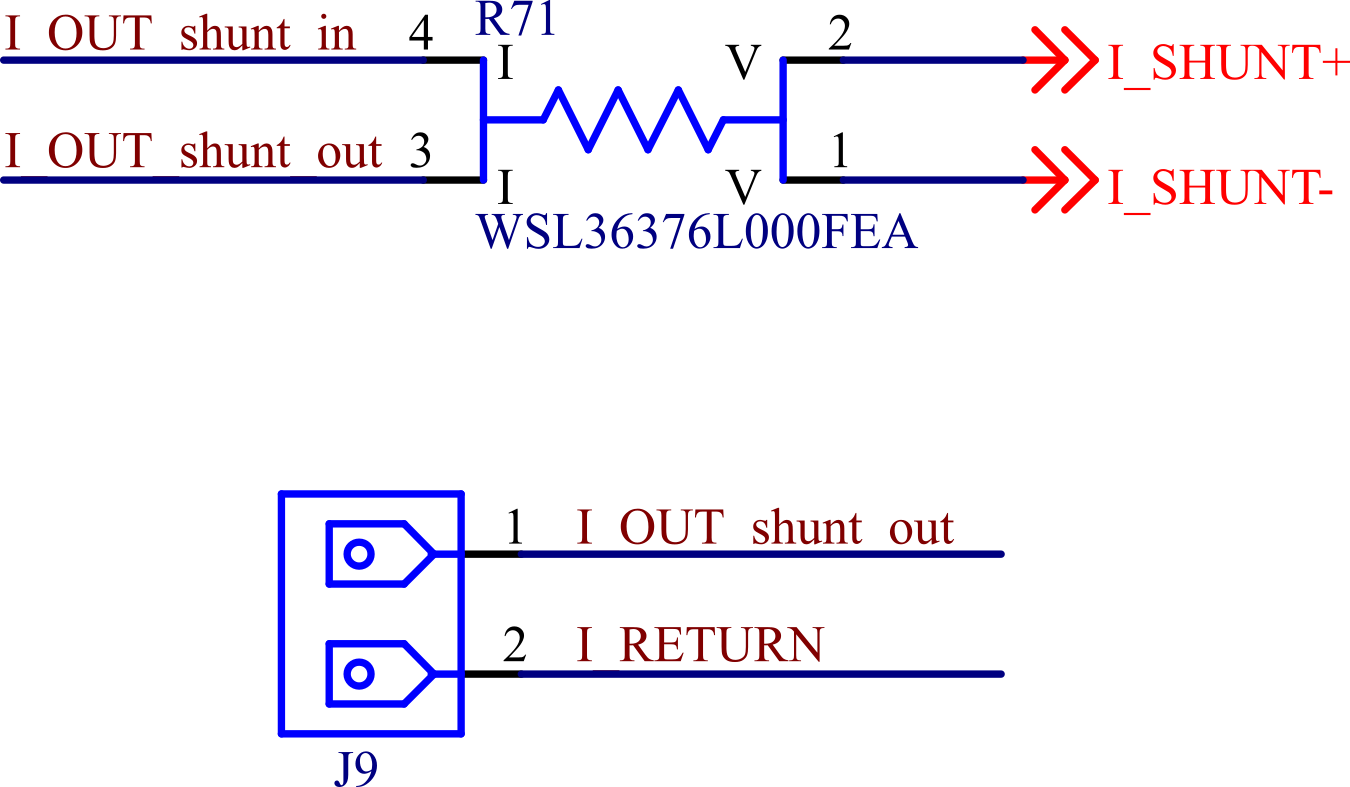
\includegraphics[width=\textwidth]{../images/mosfet-shunt.png}
    \caption{Esquemático shunt y conector}
    \label{fig:mosfet-shunt}
    \vspace*{5mm}
  \end{subfigure}
  \label{fig:generacion}
  \caption{Esquemáticos etapa de generación}
\end{figure}

  %% ----------------------------------------------------------------
  \subsubsection{Funcionamiento}
  %% ----------------------------------------------------------------
  El circuito completo a utilizar, se puede ver en la \autoref{fig:generacion-corriente}.

  \begin{figure}[!htbp]
    \centering
    \begin{circuitikz}[scale=0.6]
      \ctikzset{resistors/scale=0.55, capacitors/scale=0.55}
      \ctikzset{multipoles/thickness=3}
      \ctikzset{multipoles/dipchip/width=1.85}
      \ctikzset{transistors/scale=0.65}

      % uC
      \draw (0,0) node[dipchip, num pins=10, hide numbers, no topmark, external pins width=0](uC){$\mu$C};
      \node [right, font=\tiny] at (uC.bpin 3) {FB}; \draw (uC.bpin 3) to [short] ++(-0.5,0) \coord(uC_fb);
      \node [left, font=\tiny] at (uC.bpin 9) {PWM1}; \draw (uC.bpin 9) to [short] ++(0.5,0) \coord(uC_out1);
      \node [left, font=\tiny] at (uC.bpin 7) {PWM2}; \draw (uC.bpin 7) to [short] ++(0.5,0) \coord(uC_out2);

      % mosfet driver 1
      \draw (uC_out1) to [short] ++(1,0) \coord(md_in) to [short] ++(0.5,0) \coord(md);
      \draw (md) node[dipchip, num pins=10, hide numbers, no topmark, external pins width=0, align=center, font=\scriptsize, anchor=bpin 3] (md){MOSFET\\driver 1};
      \node [right, font=\tiny] at (md.bpin 3) {IN};
      \node [left, font=\tiny] at (md.bpin 9) {OUT1}; \draw (md.bpin 9) to [short] ++(0.5,0) \coord(md_out1);
      \node [left, font=\tiny] at (md.bpin 7) {OUT2}; \draw (md.bpin 7) to [short] ++(0.5,0) \coord(md_out2);

      % mosfets 1
      \draw (md_out1) to [short] ++(1,0) node[nigfete, anchor=G](q1){$Q_1$};
      \draw (md_out2) to [short] ++(1,0) node[nigfete, anchor=G](q2){$Q_2$};
      \draw (q1.S) -- (q2.D);
      \draw (q2.S) -- ++(0,-0.5) node[ground](GND){};

      % inductor and shunt
      \draw (q1.S) to [short, *-] ++(1,0) to [L, l=$L$] ++(2,0) -- ++(0.5,0) \coord(shunt_left) to [short] ++(0.5,0)
      to [R, l_=$R_{shunt}$] ++(1,0) to [short] ++(0.5,0) \coord(shunt_right) to [short, -*] ++(1.5,0) \coord(shunt_out);

      % mosfets 2 de arriba
      \draw (shunt_out) node[nigfete, anchor=S, xscale=-1](q3){\scalebox{-1}[1]{$Q_3$}};

      % mosfet driver 2
      \draw (q3.G) to [short] ++(1,0) \coord(md2_in) to [short] ++(0.5,0) \coord(md2);
      \draw (md2) node[dipchip, num pins=10, hide numbers, no topmark, external pins width=0, align=center, font=\scriptsize, anchor=bpin 2] (md2){MOSFET\\driver 2};
      \node [left, font=\tiny] at (md2.bpin 8) {IN}; \draw(md2.bpin 8) to [short] ++(0.5,0) \coord(md2_in);
      \node [right, font=\tiny] at (md2.bpin 2) {OUT3}; \draw (md2.bpin 2) to [short] ++(-0.5,0) \coord(md2_out3);
      \node [right, font=\tiny] at (md2.bpin 4) {OUT4}; \draw (md2.bpin 4) to [short] ++(-0.5,0) \coord(md2_out4);
      \draw (uC_out2) -| ++(0.5,-2) -| (md2_in);

      % mosfets 2 de abajo
      \draw (md2_out4) to [short] ++(-1,0) node[nigfete, anchor=G, xscale=-1](q4){\scalebox{-1}[1]{$Q_4$}};
      \draw (q4.S) -- ++(0,-0.5) node[ground](GND){};
      \draw (q4.D) -- (q3.S);

      % fuente
      \draw (q1.D) to [short] ++(0,0.5) node[vcc]{$V_{cc}$};
      \draw (q3.D) to [short] ++(0,0.5) node[vcc]{$V_{cc}$};

      % shunt medidor de tension
      \draw (shunt_left) |- ++(0.4,2) node[rmeterwashape, t=V, anchor=left](v_meter){};
      \draw (v_meter.right) -| (shunt_right);
      \draw (v_meter.center) ++(0,0.7) -- ++(0,2) -| (uC_fb);

    \end{circuitikz}
    \caption{Circuito de generación de corriente}
    \label{fig:generacion-corriente}
  \end{figure}

  El microcontrolador controlará a partir de sus salidas PWM los drivers de los MOSFETs. Así, este dictará la apertura y cierre de los cuatro MOSFET que generarán una caída de tensión sobre el multiplicador de corriente, representado en el circuito como el inductor $L$, de aproximadamente \SI{24}{V} positiva o negativa.

  Se incluirá también una resistencia de shunt $R_{shunt}$ cuya caída de tensión deberá ser medida para poder ser realimentada en el microcontrolador y así controlar la corriente generada.

  Para poder proveer las corrientes de alta frecuencia necesarias y aliviar los requerimientos sobre la fuente de tensión externa, se agregará el circuito de alimentación de la \autoref{fig:generacion-corriente-fuente}.

  \begin{figure}[!htbp]
    \centering
    \begin{circuitikz}[scale=0.7]
      \ctikzset{resistors/scale=0.6, capacitors/scale=0.6}
      \ctikzset{multipoles/thickness=3}
      \ctikzset{multipoles/dipchip/width=1.85}
      \ctikzset{transistors/scale=0.7}

      \draw (0,0) to [ecapacitor, *-, l=$C_1$] ++(0,-6) node[ground](GND){};
      \draw (0,0) -- ++(3,0) to [capacitor, *-, l=$C_2$] ++(0,-3) \coord(mid) to [capacitor, *-, l=$C_3$] ++(0,-3) node[ground](GND){};
      \draw (3,0) -- ++(3,0) to [R, -*, l=$R_1$] ++(0,-3) to [R, l=$R_2$] ++(0,-3) node[ground](GND){};

      \draw(mid) -- ++(3,0);
      \draw (3,0) to [L, l=$L_1$] ++(0,2) node[vcc](vcc){\SI{24}{V}};
      \draw (0,0) -- ++(0,0.5) node[vcc](vcc2){$V_{cc}$};

    \end{circuitikz}
    \caption{Alimentación del circuito de generación de corriente}
    \label{fig:generacion-corriente-fuente}
  \end{figure}

  El capacitor $C_1$ representará varios capacitores de film en paralelo, capaces de proveer gran cantidad de corriente en frecuencias de bajas a medias. Para la corriente agregada por el switching se agregarán capacitores cerámicos representados por $C_2$ y $C_3$. Estos proveerán las corrientes de alta frecuencia. En paralelo a estos se agregarán dos resistencias $R_1$ y $R_2$ que permitan mantener el punto medio de los capacitores cerámicos en la mitad de la tensión.

  Además de estos componentes se agregó una bobina $L_1$ que actúa de filtro pasaaltos, de manera tal que las corrientes de alta frecuencia sean obtenidas por los capacitores y no de la fuente de alimentación externa.


  %% ----------------------------------------------------------------
  \subsubsection{MOSFETs}
  %% ----------------------------------------------------------------
  Se utilizarán MOSFETs de montaje superficial, por su velocidad de conmutación, por su capacidad de disipar el calor con el mismo cobre del PCB, su baja resistencia de drain y baja resistencia térmica.

  Se montará entonces el integrado IRF3205S, que cuenta con las siguientes características:
    \begin{itemize}
      \item $V_{DSS} = \SI{55}{V}$
        \item $R_{DS_{on}} = \SI{8}{m\omega}$
        \item $I_D = \SI{110}{A}$
        \item $R_{\theta JA} = \SI{40}{\degree C/W}$
    \end{itemize}

  Como se puede observar en la \autoref{fig:mosfet}, en serie entre el driver y el MOSFET, se encuentra una resistencia en paralelo con un diodo conectado en inverso. El objetivo de la resistencia es aumentar el tiempo que tarda el transistor en encenderse, como se puede ver en la \autoref{fig:mosfet-driver-vs} obtenida del datasheet del integrado, dado que un encendido demasiado rápido puede producir tensiones negativas sobre el pin $V_S$, lo cual puede llegar a producir daños permanentes sobre el dispositivo. El diodo, por otra parte, acelera el apagado del MOSFET, previniendo las posibilidades de cortocircuito en la conmutación.

  \begin{figure}[!htbp]
    \centering
    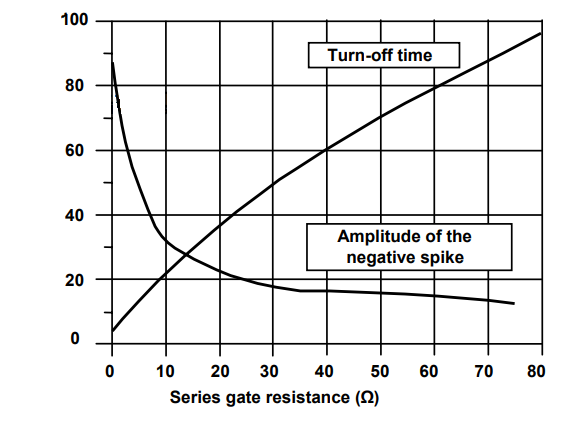
\includegraphics[scale=0.5]{../images/mosfet-driver-vs.png}
    \caption{Pico de tensión en pin $V_S$ vs. resistencia y tiempo de encendido}
    \label{fig:mosfet-driver-vs}
  \end{figure}

  %% ----------------------------------------------------------------
  \subsubsection{MOSFET driver}
  %% ----------------------------------------------------------------
  El rol de estos componentes será controlar la apertura y cierre de los MOSFET. Para ello se buscó un dispositivo que cumpliera con los requerimientos de frecuencia de switching necesarios, tensión de disparo del gate, bajo costo y de utilización general.

  El integrado que se montará será el IRS2110SPBF, de Infineon Technologies con las siguientes características:

    \begin{itemize}
      \item Tensión de gate entre \SI{10}{V} y \SI{20}{V}.
      \item Tiempo de encendido y apagado de \SI{130}{ns} y \SI{120}{ns} respectivamente.
      \item Tensión de drive del MOSFET hasta \SI{500}{V}
      \item Compatible con lógica \SI{3.3}{V}
      \item Canal flotante diseñado para utilizar con bootstrap
    \end{itemize}

  La frecuencia de switching que se utilizará es \SI{100}{kHz}, siendo el retardo del integrado despreciable comparado con esta. La tensión de gate del MOSFET será proveída por la fuente de \SI{12}{V}. Además, el MOSFET driver será disparado con el PWM del microcontrolador, de lógica \SI{3.3}{V}. Finalmente el canal flotante permitirá disparar el MOSFET del lado alto utilizando únicamente un diodo y un capacitor de bootstrap de componentes externos.

  El diagrama de bloques interno del integrado se puede ver en la \autoref{fig:mosfet-driver-bloques}.

    \begin{figure}[!htbp]
      \centering
      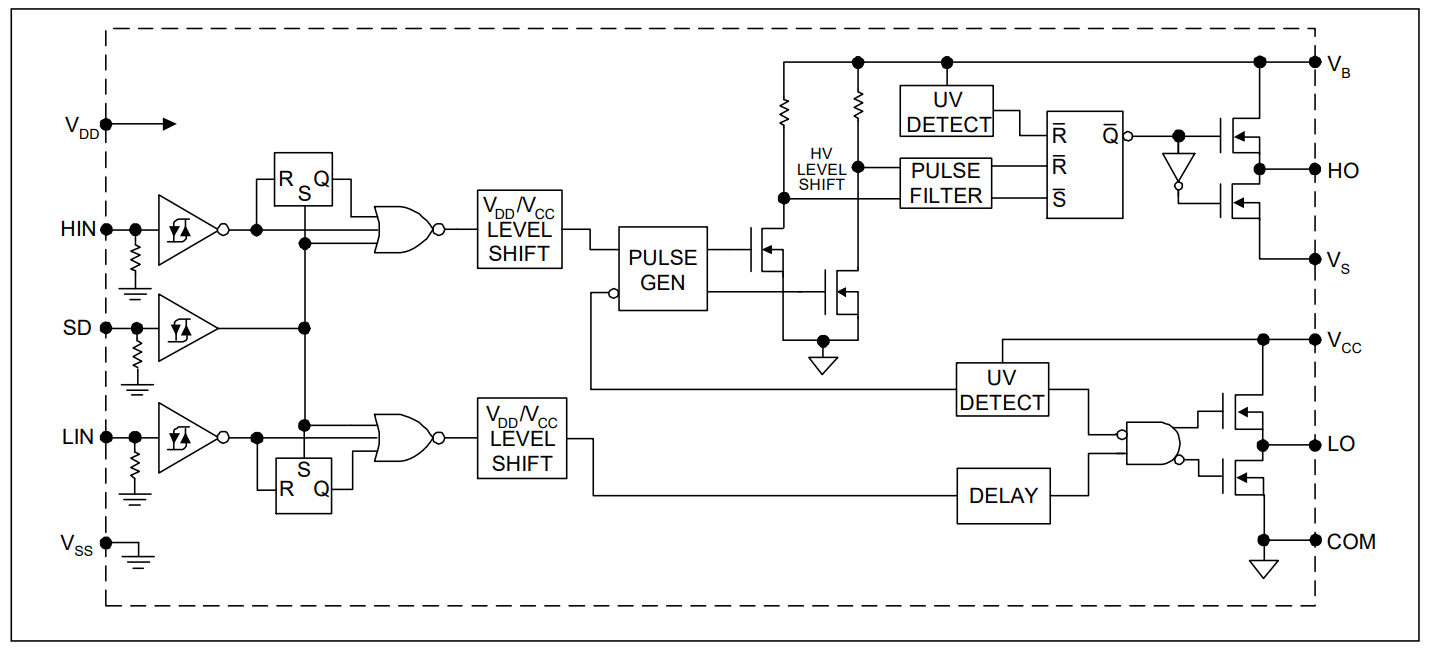
\includegraphics[scale=0.4]{../images/mosfet-driver-bloques.png}
      \caption{Diagrama en bloques del integrado IRS2110SPBF}
      \label{fig:mosfet-driver-bloques}
    \end{figure}

  Se describirá a continuación la selección realizada de componentes para el esquemático de este dispositivo.

    \paragraph{Etapa lógica} Las entradas HIN y LIN serán conectadas a los puertos PWM del microcontrolador, con dos resistencias pull-down de \SI{4.7}{k\ohm}, lo cual permitirá dejar el valor en bajo ante el apagado del microcontrolador. La fuente de tensión lógica VDD será conectada a \SI{3.3}{V}, siendo esta la máxima tensión del microcontrolador, y VSS a masa.

    \paragraph{Etapa de potencia}
    El pin de VCC se conectará a \SI{12}{V}. Los capacitores de desacople para esta pin fueron elegidos de esos valores ya que el fabricante recomienda una capacidad al menos 10 veces más grande que el capacitor de bootstrap. Se han colocado dos por motivos de disposición del PCB.

    En los pines 8 y 7 se puede ver la conexión de la fuente flotante VB y VS, el punto de retorno de la misma. El objetivo de este bloque es el de proveer una tensión mayor a \SI{24}{V} para poder activar el gate del MOSFET de la parte alta. Así, durante el período en el que el MOSFET de la parte baja está activo, el capacitor $C_{52}$ se carga a través del diodo $D_6$ a la tensión de VCC, es decir aproximadamente \SI{12}{V}. Luego cuando este MOSFET se apaga y se quiere activar el de la parte alta, VS ahora se encuentra a \SI{24}{V}, quedando la fuente flotante VB con una tensión efectiva de \SI{36}{V} debido al capacitor cargado, pudiendo así proveer la tensión necesaria al gate del MOSFET.

    \paragraph{Capacitor de bootstrap}
    Dado que el capacitor de bootstrap $C_{52}$ sera utilizado como fuente para proveer de carga al gate del MOSFET, se debe dimensionar de manera tal que mantenga su tensión luego de haberla entregado. Siguiendo las notas de aplicación brindada por el fabricante \cite{ir:an-978}, \cite{ir:dt04-04}, se han diseñado entonces los componentes de bootstrap.

  El primer paso es establecer la máxima disminución de tensión $\Delta V_{BS}$ que se puede tener en el capacitor de bootstrap $C_{bs}$ para garantizar que el MOSFET del lado alto se mantenga prendido. Esta caída estará dada por:
    \begin{equation}
      \label{eq:bootstrap-deltavbs}
      \Delta V_{BS} \leq V_{CC} - V_F - V_{GS min} - V_{DS on} - V_{Rbs}
    \end{equation}

  siendo $V_{CC}$ la tensión de la fuente de alimentación de \SI{12}{V}, $V_F$ la caída sobre el diodo de bootstrap, $V_{GS min}$ la mínima tensión de gate a mantener, $V_{DS on}$ la caída sobre el MOSFET del lado bajo cuando está encendido y $V_{Rbs}$ la caída sobre la resistencia de bootstrap. En la \autoref{fig:mosfet-driver-bootstrap} se puede observar un esquemático de esta parte del circuito.

  \begin{figure}[!htbp]
    \centering
    \begin{circuitikz}[scale=1, raised voltages]
      \ctikzset{resistors/scale=0.6, capacitors/scale=0.6, diodes/scale=0.6}
      \ctikzset{multipoles/thickness=3}
      \ctikzset{multipoles/dipchip/width=2}
      \ctikzset{transistors/scale=0.7}

      % mosfet driver
      \draw (0,0) node[dipchip, num pins=10, hide numbers, no topmark, external pins width=0, align=center, font=\scriptsize](drv){MOSFET\\driver};
      \node [right, font=\tiny] at (drv.bpin 1) {VCC}; \draw (drv.bpin 1) to [short] ++(-1,0) \coord(drv_vcc);
      \node [left, font=\tiny] at (drv.bpin 10) {VB}; \draw (drv.bpin 10) to [short] ++(0.5,0) \coord(drv_vb);
      \node [left, font=\tiny] at (drv.bpin 6) {VS}; \draw (drv.bpin 6) to [short] ++(0.5,0) \coord(drv_vs);

      % vcc
      \draw (drv_vcc) -- ++(0,-1.5) to [battery1, v_<=$V_{CC}$, invert, bipole/is voltage=false] ++(0,-2) -- ++(0,-1.5) node[ground](GND){};

      % bootstrap
      \draw (drv_vcc) to [short, *-] ++(0,2) to [R, l=$R_{bs}$, v=$V_{Rbs}$] ++(3,0) to [D*, l=D, v=$V_{F}$] ++(3,0) -- ++(0,-2) \coord(diode_out);
      \draw (diode_out) to [short, *-] (drv_vb);
      \draw (diode_out) to [C, l=$C_{bs}$, -*, v=$V_{BS}$] (diode_out |- drv_vs);

      % mosfets
      \draw (drv_vs) to [short] ++(5,0) \coord (mosfet_mid);
      \draw (mosfet_mid) -- ++(0,1) node[nigfete, anchor=S](q1){$Q_1$}; \draw (q1.D) -- ++(0,2.5) node[vcc](vcc){\SI{24}{V}};
      \draw (mosfet_mid) -- ++(0,-1) node[nigfete, anchor=D](q2){$Q_2$}; \draw (q2.S) -- (mosfet_mid |- GND) node[ground](GND){};

      % mosfet voltages
      \draw (q2.S) ++(-1.5,-0.5) \coord(q2_s);
      \draw (q2.D) ++(-1.5,0.5) to [open, v=$V_{DS on}$] (q2_s);

      % long arrow
      \draw[>=latex,->,color=MidnightBlue,text=black, thick,rounded corners=10pt]
      (drv_vcc) ++(0,3) -- ++(7.5,0) -- ++(0,-4.8) -- ++(2.25,0) -- ++(0,-1);

      \end{circuitikz}
    \caption{Esquemático de la etapa de bootstrap del MOSFET driver}
    \label{fig:mosfet-driver-bootstrap}
  \end{figure}

  Para poder encontrar $\Delta V_{BS}$, se deben hallar primero los valores de las demás tensiones, como se puede ver en \eqref{eq:bootstrap-deltavbs}. A partir de valores del fabricante y datos propios se obtuvo:
    \begin{itemize}
      \item $V_{CC} = \SI{12}{V}$
      \item $V_F = \SI{0.75}{V}$
      \item $V_{GS min} = \SI{4}{V}$
      \item $V_{DS on} = I_D \cdot R_{DS on} = \SI{10}{A} \cdot \SI{3.95}{m\ohm} = \SI{395}{mV}$
    \end{itemize}

  De aquí solo resta hallar $V_{Rbs}$. El objetivo de esta resistencia es limitar la máxima corriente que circula por el diodo $D$ al valor máximo que permite el fabricante. Para ello se calcula:
    \[
      R_{bs_{min}} = \frac{V_{CC}}{I_{D_{max}}} = \frac{\SI{12}{V}}{\SI{100}{A}} = \SI{0.12}{\ohm}
    \]
  La cual si multiplicamos por 10 para tener un margen de seguridad y redondeamos hacia arriba al valor más cercano obtenemos $R_{bs} = \SI{2}{\ohm}$, obteniendo así una corriente máxima sobre el diodo $I_{D_{max}} = \SI{6}{A}$.

  De manera de poder hallar entonces $V_{Rbs}$ en valor promedio se realiza el siguiente cálculo:
    \begin{equation}
      \label{eq:bootstrap-vrbs}
      V_{Rbs} = Q_{tot} \cdot T_{off} \cdot R_{bs}
    \end{equation}
  el cual solo podrá ser resuelto una vez se obtenga la carga total que sale del capacitor de bootstrap.

  El segundo paso es entonces, hallar todos los factores que contribuyen a que $V_{BS}$ disminuya, es decir todas las cargas y corrientes que circulan por el circuito:
    \begin{itemize}
      \item Carga de Gate requerida para encender el transistor ($Q_G$)
      \item Carga requerida por los level shifters internos del MOSFET ($Q_{LS}$), generamente 5 nC (500V/600V MOSFETs) o 20 nC (1200V MOSFETs)
      \item Corriente de fuga Gate-Source del transistor ($I_{LK-GS}$)
      \item Corriente de reposo de la sección flotante ($I_{QBS}$)
      \item Corriente de fuga de la sección flotante ($I_{LK}$)
      \item Corriente de fuga del diodo de bootstrap ($I_{LK-D}$)
      \item Corriente de desaturación del diodo encendido ($I_{DS-}$)
      \item Corriente de fuga del capacitor de bootstrap ($I_{LK-CAP}$)
      \item Tiempo que dura encendido el lado alto ($T_{Hon}$)
    \end{itemize}
  $I_{LK-CAP}$ es sólo relevante cuando se utiliza un capacitor electrolítico y puede ser ignorada si se usan de otro tipo. El fabricante recomienda utilizar al menos un capacitor cerámico con bajo ESR (puede ser en paralelo con un capacitor electrolítico).

  $I_{LK-D}$ es sólo elevante para diodos comunes, siendo en nuestro caso uno tipo Schottky.

  Entonces se tiene:
    \begin{equation}
      \label{eq:bootstrap-qtot}
      Q_{TOT} = Q_G + Q_{LS} + (I_{LK-GS} + I_{QBS} + I_{LK} + I_{LK-D} + I_{DS-}) \cdot T_{Hon}
    \end{equation}

  Para poder hallar esta carga total, se recurre a los datos de los fabricantes nuevamente, obteniendo:

    \begin{itemize}
      \item $Q_G = \SI{146}{nC}$
      \item $Q_{LS} = \SI{5}{nC}$
      \item $I_{LK-GS} = \SI{100}{nA}$
      \item $I_{QBS} = \SI{230}{\mu A}$
      \item $I_{LK} = \SI{50}{\mu A}$
      \item $I_{LK-D} = \SI{10}{mA}$
    \end{itemize}

  Se obtiene suponiendo el peor caso, cuando el MOSFET alto está el mayor tiempo prendido, es decir para $T_{Hon} = \frac{0.9}{\SI{100}{kHz}}$:

      \begin{equation}
          \label{eq:bootstrap-cmin}
          C_{bs_{min}} = \frac{Q_{TOT}}{\Delta V_{BS}} = \SI{36.22}{nF}
      \end{equation}

  Dejando un margen de seguridad de al menos 100 veces y redondeando al siguiente valor superior, se obtuvo:

    \[
      C_{bs} = \SI{4.7}{\mu F}
    \]

  %% ----------------------------------------------------------------
  \subsubsection{Protección}
  %% ----------------------------------------------------------------
  Para protección de sobrecorriente se deberá agregar el circuito mostrado en la \autoref{fig:mosfet-proteccion}. Para su diseño se utilizó el comparador LM311D, en una configuración de comparador con histéresis

  Con los valores de resistencias dados, se obtiene una histéresis de \SI{10}{A} a \SI{20}{A}.

  %% ----------------------------------------------------------------
  \subsubsection{Resistencia de shunt}
  %% ----------------------------------------------------------------
  Esta resistencia se colocará en serie al multiplicador de corriente, como se puede ver en la \autoref{fig:mosfet-shunt} de manera que deberá soportar \SI{10}{A} que circularán por esta. Se utilizará entonces la resistencia WSL36376L000FEA que tiene las siguientes características:

  \begin{itemize}
    \item $R = \SI{6}{m\Omega} \pm 1\%$
    \item $P_{max} = \SI{3}{W}$
  \end{itemize}

  Esta resistencia posee cuatro terminales, permitiendo así contar con puertos separados para la medición y la parte de potencia.

  Se deberá también incluír un conector que soporte una salida de por lo menos \SI{10}{A}, para la conexión con el multiplicador de corriente.


\end{document}
